\appendix
\section{Examples of MPS Language Aspects}
\label{sect:APX} 

The first part of this appendix contains examples of core aspects for the \code{if-then-else} statement --- Structure (Figure~\ref{fig:if_statement_structure}), Editor (Figure~\ref{fig:if_editor_definition}), and TextGen (Figure~\ref{fig:if_statement_textgen}).

\begin{figure}[ht]
\vspace{-2mm}
\centering
\begin{alltt}
\small
\mpsstkeyword{concept} IfStatement \mpsstkeyword{extends} Statement
        \mpsstkeyword{implements} IContainsStatementList

  \mpsstkeyword{instance can be root:} false
  \mpsstkeyword{alias:} \mpsstalias{if}

  \mpsstkeyword{children:}
  \mpsstproperty{condition}        : Expression[\mpsstcardinality{1}]
  \mpsstproperty{ifFalseStatement} : Statement[\mpsstcardinality{0..1}]
  \mpsstproperty{ifTrue}           : StatementList[\mpsstcardinality{1}]
  \mpsstproperty{elsifClauses}     : ElsifClause[\mpsstcardinality{0..n}]
\end{alltt}
\caption{Structure aspect of the \code{if-then-else} statement}
\label{fig:if_statement_structure}
\vspace{-4mm}
\end{figure}

Figure~\ref{fig:if_editor_definition} shows an example of what the definition of the Editor aspect for the \code{if-then-else} statement might look like.
While here we indicate positions of cell borders on each line by spaces (just for illustration), MPS GUI actually uses a graphically much more appealing way of displaying the Editor aspects, which involves vertical and horizontal lines of different colors and also background colors other than white for some cells.
The symbols \verb|[-| and \verb|-]| represent layout information, which specifies mutual positioning of the contained cells (vertical, horizontal, indentation).

\begin{figure}[ht]
\vspace{-1mm}
\centering
\begin{alltt}
\small
\mpsedannotation{<default>} \mpsedkeyword{editor for concept} \mpsedtarget{IfStatement}
  \mpsedkeyword{node cell layout:}
    [-
      \mpsedkeyword{if} \textbf{(} \% conditions \% \textbf{)} [-
      \textbf{\{}
      [- \% ifTrue % -]
      \textbf{\}}
      -]
      ?[- \mpsedkeyword{else} \% ifFalseStatement \% -]
    -]
\end{alltt}
\vspace{-1mm}
\caption{Editor aspect for the \code{if-else} statement}
\label{fig:if_editor_definition}
\vspace{-2mm}
\end{figure}

TextGen aspect for each AST node (concept of the language) has to be defined using the BaseLanguage.
The definition follows a straightforward pattern --- each node outputs its textual representation into a buffer, while calling TextGen of its children nodes.
MPS calls the corresponding method on the root AST nodes of the given program.
Figure~\ref{fig:if_statement_textgen} shows an example for the \code{if-else} statement.

\begin{figure}[ht]
\vspace{-2mm}
\centering
\begin{alltt}
\small
\mpstgkeyword{text gen component for concept} \mpstgtarget{IfStatement} \{
  \mpstgparam{(context, buffer, node)->void} \{
    \mpstgaction{append} \textcolor{blue}{\textbf{\textbackslash{}n;}}
    \mpstgaction{indent buffer;}
    \mpstgaction{append} \{\mpstgliteral{if (}\} \$\{\mpstgparam{node}.\mpstgnodeprop{condition}\} \{\mpstgliteral{) \{}\};
    \mpstgkeyword{with indent} \{
      \mpstgaction{append} \$\{\mpstgparam{node}.\mpstgnodeprop{ifTrue}\};
    \}
    \mpstgaction{append} \textcolor{blue}{\textbf{\textbackslash{}n}} \{\mpstgliteral{\}}\} \$list\{\mpstgparam{node}.\mpstgnodeprop{elsifClauses}\};
    \mpstgkeyword{if} (\mpstgparam{node}.\mpstgnodeprop{ifFalseStatement}.\textbf{isNotNull}) \{
      \mpstgaction{append} \{ \mpstgliteral{else}\} \$\{\mpstgparam{node}.\mpstgnodeprop{isFalseStatement}\};
    \}
  \}
\}
\end{alltt}
\vspace{-1mm}
\caption{TextGen aspect definition for the \code{if-else} statement}
\label{fig:if_statement_textgen}
\vspace{-2mm}
\end{figure}

Figure~\ref{fig:EDITORADJUST} shows the Editor aspect for the \mpsconcept{Element{\_}1} concept --- the basic, automatically generated, layout in the upper left corner and a fully customized layout in the bottom right part.

\begin{figure*}[ht]
	\centering
	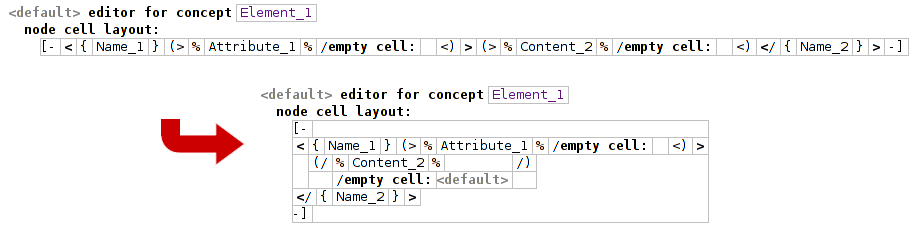
\includegraphics[scale=0.55]{./images/editor_adjustment.png}
	\caption{Editor aspect of the \mpsconcept{Element{\_}1} concept}
	\label{fig:EDITORADJUST}
\end{figure*}

Figure~\ref{fig:TEXTGENFINAL} contains the complete, automatically generated, TextGen aspect for the \mpsconcept{Element{\_}1} concept.
Such code may be adjusted by hand very easily in order to produce nicely indented XML documents.
We only need to wrap the \mpsconcept{Content{\_}2} child node with indentation and change the sequence separator to a new line character.
A fragment of the resulting adjusted code is in Figure~\ref{fig:TEXTGENADJUSTED}.

\begin{figure}[ht]
\vspace{-2mm}
\begin{alltt}
\small
\mpstgkeyword{text gen component for concept} \mpstgtarget{Element{\_}1} \{
  \mpstgparam{(context, buffer, node)->void} \{
    \mpstgaction{append} \{\mpstgliteral{<}\};
    \mpstgkeyword{if} (\mpstgparam{node}.\mpstgnodeprop{\textit{Name}}{\_}\textit{1}.\textbf{isNotEmpty}) \{
      \mpstgaction{append} \$\{\mpstgparam{node}.\mpstgnodeprop{\textit{Name}}{\_}\textit{1}\};
    \}
    \mpstgkeyword{if} (\mpstgparam{node}.\mpstgnodeprop{\textit{Attribute}}{\_}\textit{1}.\textbf{size} > 0) \{
      \mpstgaction{append} \{\ \};
      \mpstgaction{append} \$list\{\mpstgparam{node}.\mpstgnodeprop{\textit{Attribute}}{\_}\textit{1} with  \};
    \}
    \mpstgaction{append} \{\mpstgliteral{>}\};
    \mpstgkeyword{if} (\mpstgparam{node}.\mpstgnodeprop{\textit{Content}}{\_}\textit{2}.\textbf{size} > 0) \{
      \mpstgaction{append} \$list\{\mpstgparam{node}.\mpstgnodeprop{\textit{Content}}{\_}\textit{2} with  \};
    \}
    \mpstgaction{append} \{\mpstgliteral{</}\};
    \mpstgkeyword{if} (\mpstgparam{node}.\mpstgnodeprop{\textit{Name}}{\_}\textit{2}.\textbf{isNotEmpty}) \{
      \mpstgaction{append} \$\{\mpstgparam{node}.\mpstgnodeprop{\textit{Name}}{\_}\textit{2}\};
    \}
    \mpstgaction{append} \{\mpstgliteral{>}\};
  \}
\}
\end{alltt}
\caption{Full TextGen aspect for the \mpsconcept{Element{\_}1} concept}
\label{fig:TEXTGENFINAL}
\vspace{-1mm}
\end{figure}

\begin{figure}[ht]
\begin{alltt}
\small
\mpstgkeyword{if} (\mpstgparam{node}.\mpstgnodeprop{\textit{Content}}{\_}\textit{2}.\textbf{size} > 0) \{
  \mpstgaction{append} \textcolor{blue}{\textbf{\textbackslash{}n;}}
  \mpstgaction{indent buffer;}
  \mpstgkeyword{with indent} \{
    \mpstgaction{append} \$list\{\mpstgparam{node}.\mpstgnodeprop{\textit{Content}}{\_}\textit{2} with  \};
  \}
  \mpstgaction{append} \textcolor{blue}{\textbf{\textbackslash{}n;}}
\} 
\end{alltt}
\vspace{-1mm}
\caption{Fragment of the TextGen aspect of \mpsconcept{Element{\_}1} with adjusted indentation}
\label{fig:TEXTGENADJUSTED}
\vspace{-2mm}
\end{figure}

